% ------------------------------------------------------------------- %
% ------------------------------------------------------------------- %
\chapter{Overview}
\label{sec:overview}

The goal of this chapter is to give an overview of the theoretical and algorithmic pieces needed to understand the inputs for, and outputs of MORIS' mesh generation workflow.
%This chapter will lay out the some pieces of theory that are beneficial to understanding the mesh generation and its output. 
As mentioned in the foreword, the output data is intended to perform interpolation-based immersed finite element analysis, the theory for which, with the exception of a brief introduction to \hyperref[sec:overview_extraction]{Lagrange extraction}, will not be discussed in this document. Instead the reader is advised to consult the publication by Fromm et al. \cite{Fromm2022}

\refpar{moris_overview}{MORIS} ("Multi-physics Optimization Research and Innovation System") is a standalone finite element and topology optimization software framework. The analysis method utilized inside MORIS itself is a quadrature-based immersed isogeometric method. The interpolation function basis is provided by a rectangular \hyperref[sec:overview_background]{tensor-product B-spline mesh}, the \textbf{background mesh}, that can be \hyperlink{hierarchical_refinement}{hierarchically refined}. Next, geometries are immersed into said mesh. The geometry is described implicitly by \hyperref[sec:overview_geometry]{level-set fields} $\Phi(\bm{x})$ and their iso-contours  $\Phi(\bm{x}) = c$. A quadrature rule for evaluating the discretized weak form is found by tessellating, or \hyperlink{decomposition}{"\emph{decomposing}"}, the background mesh's elements intersected by the iso-contours into triangles or tetrahedrons whose Gauss points and weights provide the integration rule. Additionally, the background basis is \hyperlink{enrichment}{Heaviside enriched} to solve problems involving multiple materials. For the interested reader, the isogeometric analysis framework inside MORIS is explained in more detail by No\"el et al. \cite{Noel2022} and Schmidt et al. \cite{Schmidt2022}.

The set of non-intersected background elements and triangular elements within intersected elements together form a body-fitted mesh which from here on will be referred to as the \textbf{foreground mesh}. This body-fitted foreground mesh and its known relation to the background mesh together form the mesh information needed for interpolation-based immersed analysis. Hence, the mesh generation abilities of MORIS can directly be exploited to provide all mesh information needed to perform interpolation-based immersed finite element analysis.

The meshing apparatus inside MORIS consists of three modules: a hierarchical B-spline mesh generator called HMR, a geometry engine (GEN), and an extended finite element tool kit (XTK). To obtain the desired meshes, the inputs for these three modules need to be configured. More specifically, HMR needs to be fed what the size, dimensions, and order of its tensor-product meshes is, and how they're to be refined. GEN needs level-set fields to determine interface locations and material membership. XTK works based off the information provided by the other modules, apart from minor configuration input. A \hyperref[fig:workflow]{chart of the workflow} is shown below.

\vspace*{0.5cm}

\begin{figure}[h]
    \vspace{0.5cm}
    \begin{center}
    %\def\svgwidth{15.0cm}
    \input{Figures/workflow.pdf_tex}
    \caption{Workflow for mesh generation inside MORIS} 
    \label{fig:workflow}
    \end{center}
\end{figure}

The remainder of this chapter is structured as follows. First, a short introduction on how \hyperref[sec:overview_geometry]{geometries} can be defined with level-set fields will be given. Next, the \hyperref[sec:overview_background]{interpolation basis} used by MORIS is defined alongside the \hyperlink{enrichment}{enrichment strategy} used. Lastly, the \hyperlink{decomposition}{algorithm for generating the foreground mesh} is shown and how the \hyperref[sec:overview_extraction]{extraction operators} are computed from it.

\paragraph{Note:} The features currently supported in the pure mesh generation workflow do not include all features supported by MORIS internally, but are undergoing expansion to do so. Until then, some parts of this chapter may seem unnecessary. 

% \hyperref[sec:overview_workflow]{workflow}
% \hyperlink[enrichment]{enrichment}

% ------------------------------------------------------------------- %
\section{Geometry}
\label{sec:overview_geometry}

As mentioned above, geometry in MORIS is described implicitly by a level-set field $\Phi_i(\bm{x})$ and a threshold $c$, which is assumed to be $c=0$ from here on, determining the locations of interfaces. 
This leads to a natural definition of what is \emph{inside} and \emph{outside} a given geometry. 

\begin{equation}
\label{eq:level_set_field}
    \Phi_i(\bm{x}) 
    \begin{cases}
        < 0 & \bm{x} \notin \Omega_i \\
        = 0 & \bm{x} \in \partial\Omega_i \\
        > 0 & \bm{x} \in \Omega_i \\
    \end{cases}
\end{equation}

\hypertarget{phase_assignment}{}
If multiple level-set fields, and therefore geometries, are introduced, each point $\bm{x}$ is defined to be either inside or outside with respect to each of the geometries. Each region of points that is a certain combination of inside/outside with respect to each of the geometries is called a \emph{phase}. This leads to there being up to $n_p = 2^{n_{LSF}}$ phases inside a given domain, when $n_{LSF}$ geometries are defined. \emph{Material} sub-domains can simply be defined by merging these phases, as illustrated in \Cref{fig:phase_mergin}

\begin{figure}[h]
    \begin{center}
    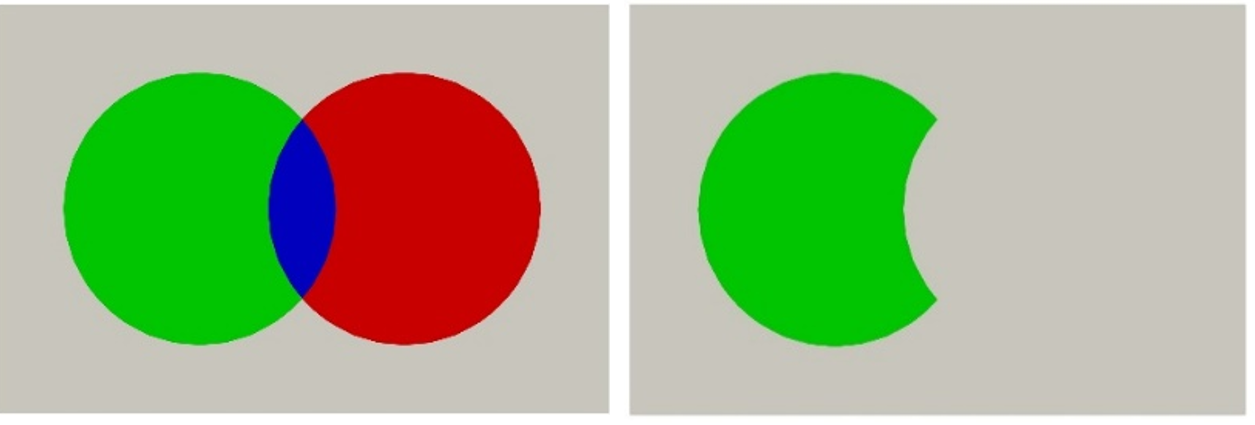
\includegraphics[width=10cm]{Figures/phase_merging.png}
    \caption{Introducing two discs as geometries into an ambient domain results in four phases (marked in different colors). Material domains can be defined by merging phases. } 
    \label{fig:phase_mergin}
    \end{center}
\end{figure}

A particularly notable type of level-set field is a so-called signed-distance field, which every point has a value whose magnitude corresponds to the minimum distance to an interface.
Any geometry definition that has a notion of "inside" and "outside" can be converted to a signed-distance field and therefore be used with MORIS, if a pre-processor for the conversion exists.

% ------------------------------------------------------------------- %
\section{Background Basis and Enrichment}
\label{sec:overview_background}

\paragraph{Tensor-Product B-spline Basis}
B-spline basis functions are used to define the function basis of the background mesh. 
The B-spline basis functions $N_{i,p}$ of polynomial order $p$ are defined by a knot vector $\left\{\xi_i\right\}_{i = 1}^{n}$ containing a set of control points, and the Cox-de Boor recursive formula.  The definition of the $i$-th basis function starts with piece-wise constant parts for zeroth order $p=0$ B-spline basis function.

\vspace*{0.3cm}

\begin{equation} 
\label{eqn:BasisP0}
    N_{i,0}(\xi) = 
    \left\{
    \begin{array}{ll}1 \ if \ \xi_i \leq \xi < \xi_{i+1}\\  0\ else\end{array}
    \right.
\end{equation} 

B-spline basis functions of higher order can be constructed by evaluating the following equation recursively:
    
\begin{equation}
\label{eqn:CoxBoor}
    N_{i,p}(\xi) = 
    \frac{\xi - \xi_i}{\xi_{i+p} - \xi_i} N_{i,p-1}(\xi) + 
    \frac{\xi_{i+p+1} - \xi}{\xi_{i+p+1} - \xi_{i+1}} N_{i+1,p-1}(\xi)
\end{equation}

This recursive definition leads to a piece-wise polynomial definition of the basis functions. 

\begin{figure}[H]
    % \vspace{0.2cm}
    \begin{center}
    \def\svgwidth{13.0cm}
    \input{Figures/BSp_Basis.pdf_tex}
    \caption{$C^{p-1}$ continuous B-spline basis functions constructed from unique and uniform knot vectors or orders $p = {1,2,3}$ defining an interpolation basis for the computational domain $\mathcal{A} = [1,3]$} 
    \label{fig:Bsp_basis}
    \end{center}
\end{figure}

Using a knot vector of unique and equispaced control points $\xi_i$ results in \textbf{$C^{p-1}$ continuous} basis functions that are translated and repeated. The intervals between the control points can be considered elements (i.e. \textbf{the control points act as mesh lines}), as in each of these regions a unique set of $p+1$ basis functions interpolate into. With exception of the first and last $p$ knot intervals, called the \emph{padding}, each of these sets of basis functions form a complete polynomial basis and a partition of unity. Hence, the padding is not part of the ambient domain $\mathcal{A}$ on which a complete interpolation basis is defined. The polynomial basis and the domain they cover is shown in \Cref{fig:Bsp_basis}. A notable feature of basis functions defined this way is their \textbf{increasing support size for increasing polynomial orders} $p$.

The definition of the basis is extended into multiple ($d$) spatial dimensions by forming tensor products from these basis functions.

\begin{equation}
\label{eqn:tensor_product}
    N_{i_1, \cdots, i_d}(\bm{\xi}) = \prod_{d}^{n_d}N_{i_d}(\xi_d)
\end{equation}

The basic tensor-product B-spline basis used inside MORIS is constructed from an equispaced grid whose mesh lines represent the unique control points used to define the B-spline basis functions in each spatial dimension.

\paragraph{Hierarchical Refinement}
\hypertarget{hierarchical_refinement}{}

H-refinement could be performed by inserting additional knot points and therefore mesh lines. However, this would the additional mesh lines created would propagate throughout the whole domain.
Instead, a hierarchical basis definition is employed to perform local refinement of the tensor-product B-spline background mesh.

\begin{figure}[H]
    \centering
    \begin{minipage}{0.5\textwidth}
        \centering
        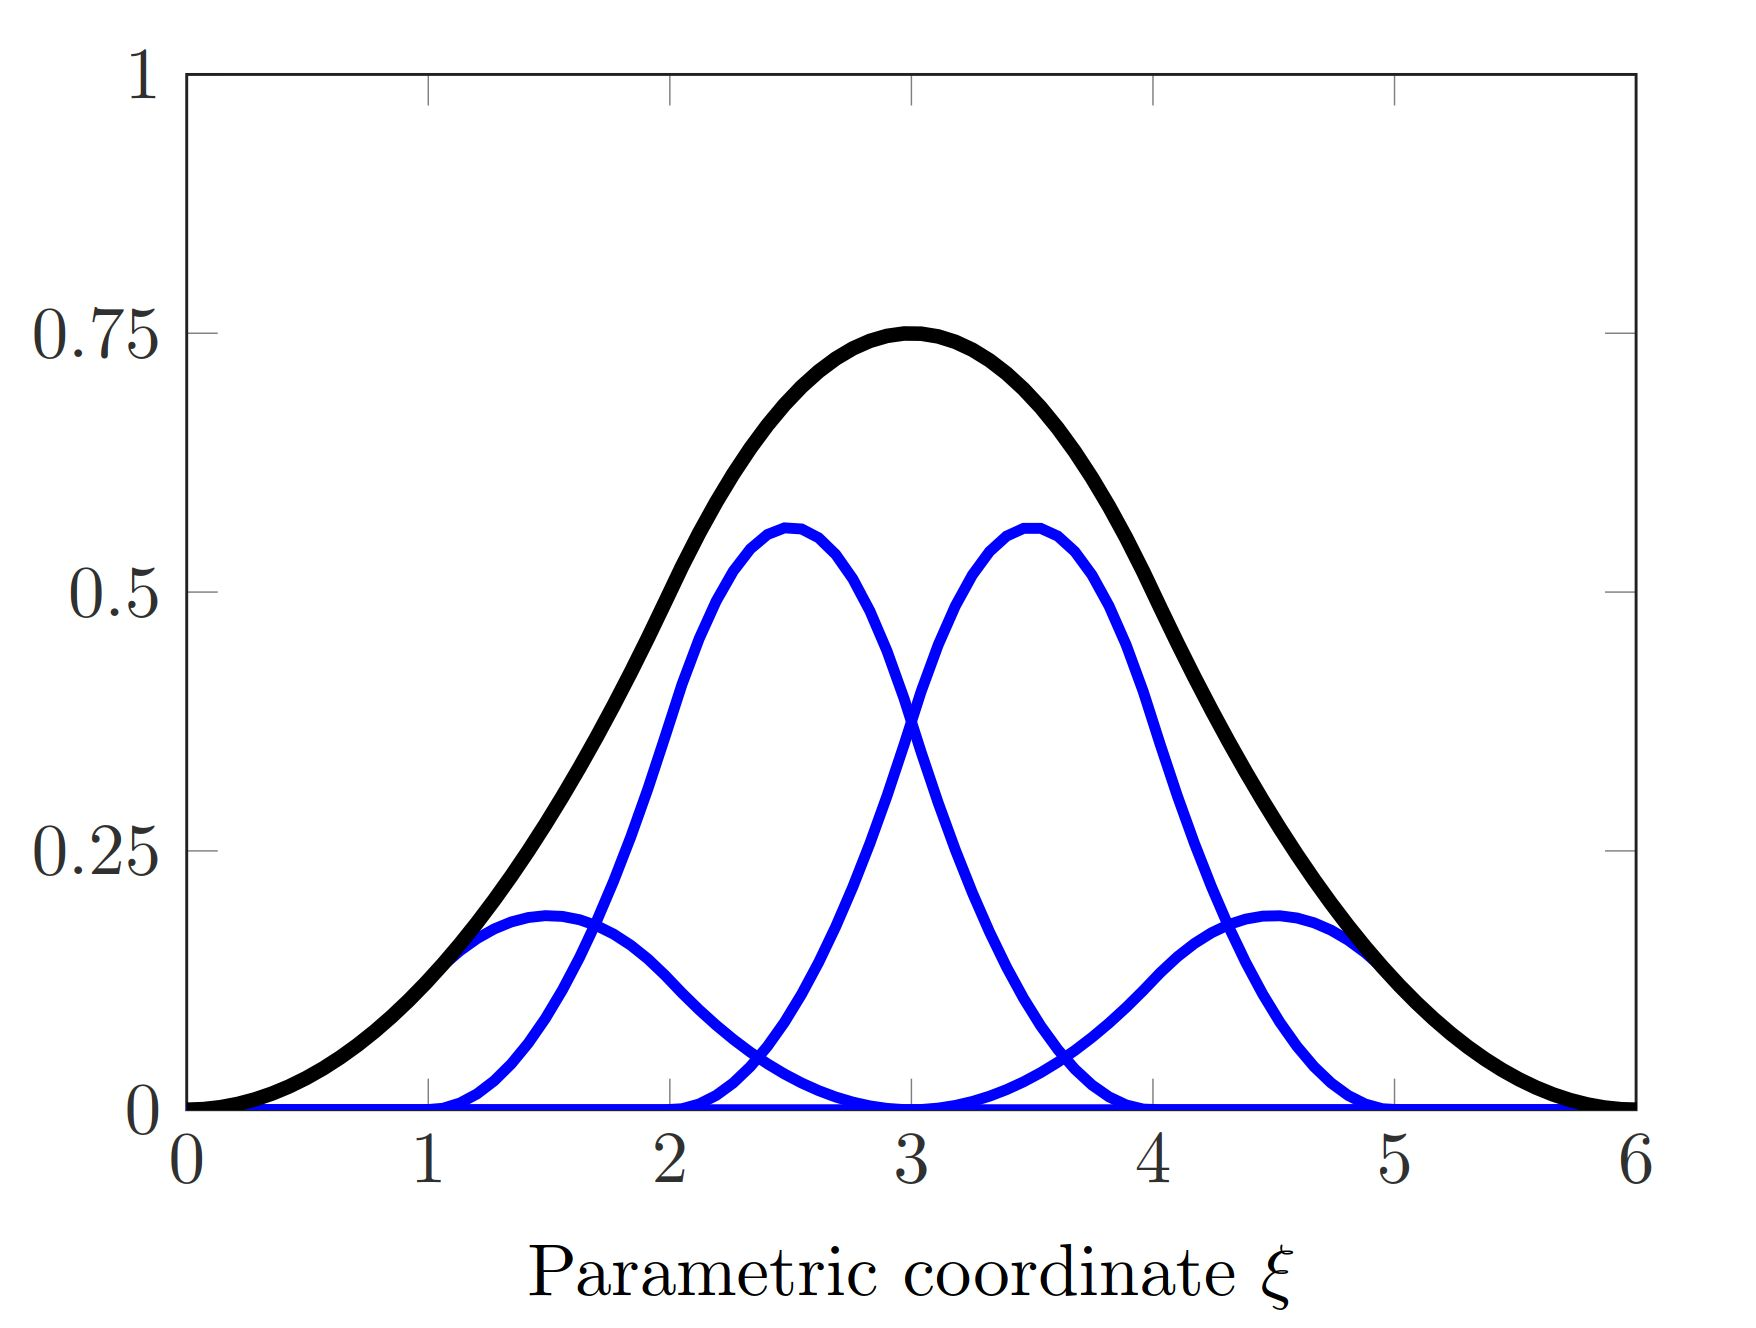
\includegraphics[width = 7.5cm]{Figures/truncation.jpg}
        \caption{The black basis function is a \\ sum of the blue translated, \\ scaled, and weighted versions \\ of itself. }
        \label{fig:truncation}
    \end{minipage}%
    \begin{minipage}{0.5\textwidth}
        \centering
        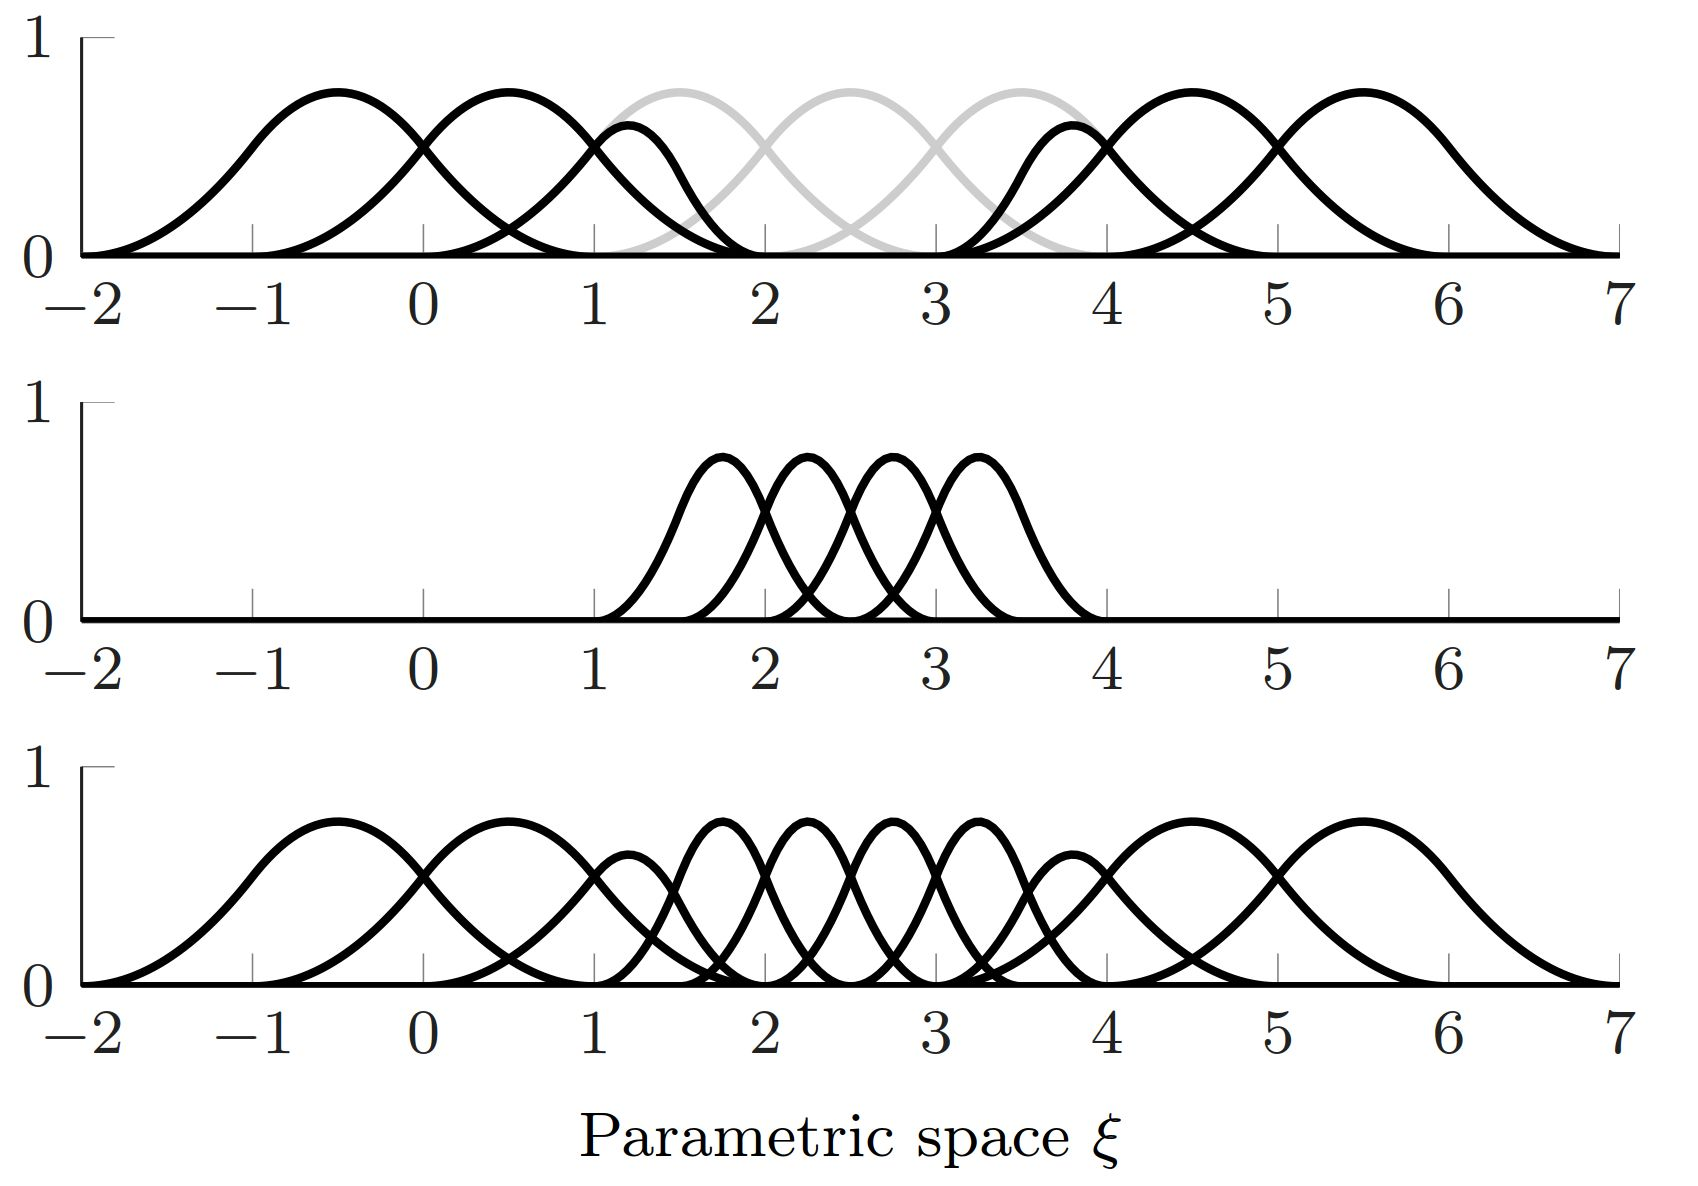
\includegraphics[width = 7.8cm]{Figures/thb_basis.jpg}
        \caption{Construction of a 1D hierarchical \\ B-spline basis. }
        \label{fig:thb_basis}
    \end{minipage}
\end{figure}

Each B-spline basis function can be represented as a sum of translated, scaled and weighted versions of itself, like shown in \Cref{fig:truncation}. These \emph{finer} versions of a \emph{coarse} basis function are constructed from the coarse knot vectors that have additional knots inserted at the midpoints of their knot intervals.

This allows a coarse basis function at a refinement level $l$ to be replaced by a weighted set of basis functions of refinement level $l+1$. The underlying tensor-product elements can be understood to undergo \textbf{quadtree or octree refinement} due to the introduction of additional mesh lines splitting them into four or eight elements in 2D and 3D respectively.

The domain of the elements on a given \emph{level} $l$ marked for refinement is denoted as $\Omega^{l+1}$. On this domain $\Omega^{l+1}$, e.g. the single element domain $\Omega^{1} = [2,3]$ shown in \Cref{fig:thb_basis}, a set of finer basis functions interpolating into it is constructed on the refined level $l+1$. Assuming that all coarse basis functions $N^l$ are represented by a weighted sum of finer basis functions $N^{l+1}$, the contribution of the finer basis functions actually constructed can be subtracted from them. This leads to either \textbf{truncation} or removal of the coarse basis functions as shown in the top row of \Cref{fig:thb_basis}. The definition of the resulting truncated coarse basis functions can be stated as:
\begin{equation}
\label{eqn:truncation}
\begin{split}
    trunc^{l+1}(N^l) = \sum_{j: N_j \nsubseteq \Omega^{l+1}} \alpha_j N_j^{l+1}
\end{split}{}
\end{equation}{}

The new, locally refined basis is the sum of the constructed fine basis and truncated coarse basis, as shown in the third row of \Cref{fig:thb_basis}. The truncated hierarchical basis can be stated as a sum of recursively defined components:

\begin{equation}
\label{eqn:thb_basis}
\begin{split}
    %\mathcal{T}^0 \ \ &= \ \mathcal{B}^0 \\
    &\mathcal{V}^{h} = \bigcup_{l=0}^{L} \mathcal{V}^{l} \\
    where ~~~\mathcal{V}^{l+1} &= \left\{ trunc^{l+1}(N) \ | \ B \in \mathcal{V}^l \land supp(N) \nsubseteq \Omega^{l+1}  \right\} \\
    & \ \ \ \ \cup \left\{ N \in \mathcal{V}^{l+1} \ | \ supp(N) \subseteq \Omega^{l+1}  \right\}
\end{split}{}
\end{equation}{}

where $\mathcal{V}^{0}$ is the tensor-product B-spline basis described at the \hyperref[sec:overview_background]{beginning of this section}.

\begin{figure}[H]
    \centering
	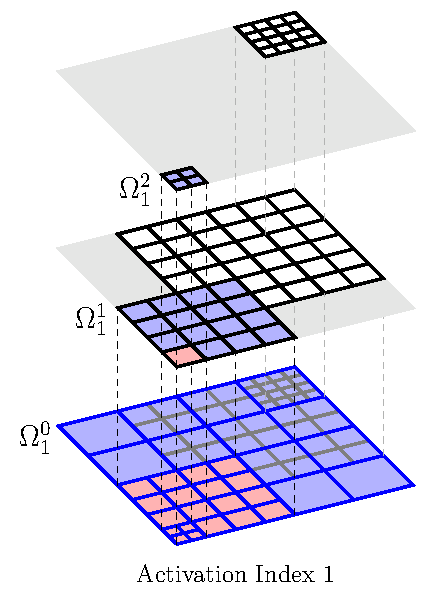
\includegraphics[width=0.32\columnwidth]{Figures/fig_hMesh1}\hspace{0.34cm}
	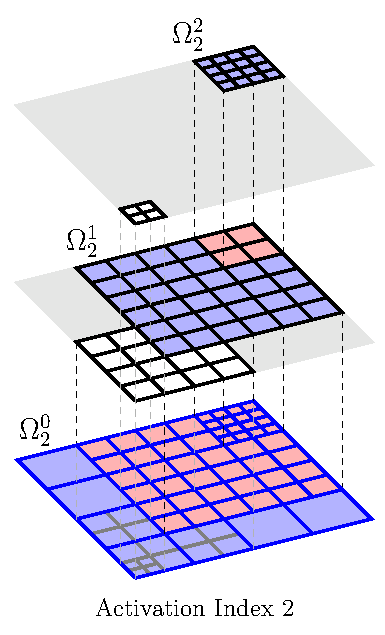
\includegraphics[width=0.30\columnwidth]{Figures/fig_hMesh2}
	\caption{Definition of multiple background mesh grids by marking sub-domains $\Omega_{i}^{l}$ for refinement.}
	\label{fig:hierarchical_refined_mesh}
\end{figure}

MORIS enables multiple hierarchically refined B-spline meshes to be created by refining a single mesh grid in different ways, like shown in \Cref{fig:hierarchical_refined_mesh}. Additionally, B-spline basis functions of various polynomial degrees $p$ can then be defined on the resulting grids.

\paragraph{Enrichment}
\hypertarget{enrichment}{}

Individual B-spline elements may contain multiple materials within them. Meanwhile, the state variable fields within these materials are decoupled. This is achieved by employing a generalized Heaviside enrichment strategy. 

For each basis function $N_j(\bm{x})$ a set of degrees of freedom (DoFs) $\left\{d_{j}^{e}\right\}_{e=1}^{n_e}$ are introduced. Indicator functions $\psi_{j}^{e}(\bm{x})$ provide the information whether a combination of DoF and basis function is active or $=0$ at a given point $\bm{x}$. 

\begin{equation}
\label{eqn:enrichment}
    u^h(\bm{x}) = \sum_{j = 1}^{n_B} \sum_{e = 1}^{n_{e,j}} \psi_{j}^{e}(\bm{x}) \cdot N_j(\bm{x}) \cdot d_{j}^{e}
\end{equation}{}

The index $e$ would traditionally correspond to the material index of a given point. However, for small scale features, like the protrusion shown in \Cref{fig:basis_function_enrichment} (a), artificial coupling in the solution between the material regions on either side of it could still be observed due to the same basis B interpolating into either separated region.

\begin{figure}[H]
    \centering
	\centering
	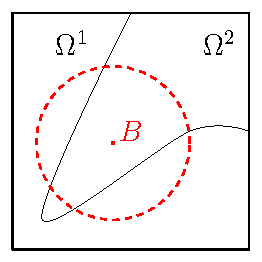
\includegraphics[width=0.23\textwidth]{Figures/fig_enrichment.pdf}
	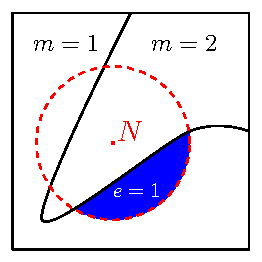
\includegraphics[width=0.23\textwidth]{Figures/fig_enrichment1.pdf}	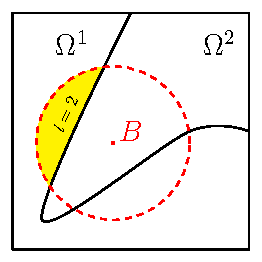
\includegraphics[width=0.23\textwidth]{Figures/fig_enrichment2.pdf}
	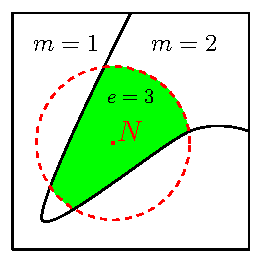
\includegraphics[width=0.23\textwidth]{Figures/fig_enrichment3.pdf}
	\caption{ Basis function enrichment for a two material problem. The support of a basis function $B$ with arbitrary support is illustrated in red. The basis function is enriched three times based on the three topologically disconnected regions of the two materials it is interpolating into.}
	\label{fig:basis_function_enrichment}
\end{figure}

To alleviate this issue, MORIS considers the material layout within a given basis functions support. Enrichment levels $e$ and corresponding DoFs $d_{j}^{e}$ are created for each disconnected material region within the support. This implies that a different set of non-zero B-spline basis functions interpolates into a point on a material interface depending not only on the material index with respect to which it is considered, but also the material layout in its vicinity. An example is provided by \Cref{fig:basis_function_enrichment}.

% ------------------------------------------------------------------- %
\section{Foreground Mesh}
\label{sec:overview_foreground}

As mentioned in the \hyperlink{moris_overview}{overview of MORIS}, the foreground mesh is generated by decomposing the background mesh, or more precisely one of the background grids. This process will be referred to as the \emph{decomposition}.

\refpar{decomposition}{The Decomposition} consists of the following steps which are also visualized in \Cref{fig:decomposition}
\begin{itemize}
    \item The first step is to identify which particular background elements are intersected and need to be decomposed. To do so, the values of all level-set fields $\Phi_i(\bm{x})$ are checked at the vertices, i.e. the "corners", of the background element. If a sign change is detected between level-set values, the element is marked for decomposition. Note, due to this particular way of intersection detection, material regions completely contained within a single background element, or protrusions through individual facets may not be detected.

    \item \hypertarget{regular_subdivision}{In a next step,} each intersected background element is subdivided into triangles or tetrahedrons, depending on dimensionality. This step will be referred to as the \emph{regular subdivision}.

    \item The edges of the triangular elements created in the regular subdivision can again be checked for sign changes in the level-set fields. Depending on which edges of a given triangle or tetrahedron are intersected, the element can be further subdivided into a pre-defined set of triangles or tetrahedrons.
    This step is subsequently repeated for each geometry in the order that the level-set fields are defined. Hence, the resulting foreground mesh may differ slightly depending on the order in which the level-set fields are defined.
    
    \item At this point the elements are just geometric entities. By placing nodes at the vertices linear elements are obtained. Higher order elements are obtained by positioning equispaced (with respect to a standardized parametric element) nodes along the edges and the inside of the resulting triangles and tetrahedrons.
    
    \item All elements are assigned a material membership based on the signs of the level-set functions, as \hyperlink{phase_assignment}{discussed previously}.
\end{itemize}

\begin{figure}[h]
    \vspace{0.2cm}
    \begin{center}
    %\def\svgwidth{15.0cm}
    \input{Figures/decomposition.pdf_tex}
    \caption{Decomposition of a background mesh grid into a geometry-fitted foreground mesh.} 
    \label{fig:decomposition}
    \end{center}
\end{figure}

\vspace{0.5cm}

The \hyperlink{decomposition}{decomposition process} layed out above leads to a foreground mesh with the \hypertarget{foreground_mesh_properties}{properties} listed below.
\begin{itemize}
    \item The element facets created during the templated triangulation are straight. Therefore, the \textbf{approximation of the geometry is piecewise linear}.
    
    \item Since the foreground mesh constructed by decomposition of a background grid, it is \textbf{background-fitted} as defined by Fromm et al. \cite{Fromm2022}.
    
    \item Further, the \textbf{quality of the geometry approximation is influenced by the resolution of the background grid} that is decomposed. Quadtree or octree refinement around the interfaces may be performed to improve the geometry representation.
    
    \item The simple algorithmic decomposition may lead to \textbf{triangular elements of extremely poor quality} (large aspect ratios, very high maximum angles). For interpolation-based immersed analysis the poor element quality is generally not of concern though.

    \item Non-intersected quadrilateral or hexahedral background elements are not decomposed. The resulting foreground mesh therefore contains a \textbf{mix of triangular and rectangular elements}. Non-intersected elements may additionally be marked for regular subdivision, though.

    \item If a hierarchically, i.e. locally, refined background mesh grid is used for decomposition, the \textbf{foreground mesh may contain hanging nodes}, like shown in \Cref{fig:decomposition}.
\end{itemize}

% ------------------------------------------------------------------- %
\newpage
\section{Lagrange Extraction}
\label{sec:overview_extraction}

Lastly, it should be useful to recap the basics of Lagrange extraction. 
The key to performing interpolation-based analysis is the fact that Lagrange basis functions $\phi_j(\bm{x})$ are \emph{interpolatory}, i.e. they are $=1$ at exactly one nodal point, and $=0$ at every other nodal point $\hat{\bm{x}}_i$. An illustration for linear Lagrange basis function inside a linear triangular element is provided on the right of \Cref{fig:lagrange_extraction}.

\begin{equation}
\label{eq:interpolatory}
    \phi_i(\hat{\bm{x}}_i) =
    \left\{
    \begin{array}{@{}c@{}}
        1 ~~~ j=i \\
        0 ~~~ j \neq i
    \end{array} 
    \right\} 
    = \delta_{ij}
\end{equation}
    
\begin{figure}[h]
    \vspace{0.2cm}
    \begin{center}
    %\def\svgwidth{15.0cm}
    \input{Figures/Lagrange_basis_functions.pdf_tex}
    \caption{Lagrange extraction.} 
    \label{fig:lagrange_extraction}
    \end{center}
\end{figure}

A Lagrange element can be placed into another mesh that may provide another type of interpolation $u^{h,B} = \sum_{j=1}^{n_B} N_j(\bm{x}) \cdot d_j$. The two interpolations $u^{h}$ can be assumed to be approximately equal to each other (in a mathematically crude fashion).

\begin{equation}
\label{eq:approx}
\begin{split}
    u^{h,B} 
    &\approx u^{h,L} \\
    \sum_{j=1}^{n_B} N_j(\bm{x}) \cdot d_j 
    &\approx \sum_{i=1}^{\nu} \phi_j(\bm{x}) \cdot c_j
\end{split}
\end{equation}

Substituting identity \eqref{eq:interpolatory} into the equation at the nodal points $\hat{\bm{x}}_i$ yields the extraction operator $M_{ij}$ relating the degrees of freedom of the two bases to each other.

\begin{equation}
    \label{eq:derive_extraction_operator}
    \begin{split}
        \sum_{j=1}^{n_B} N_j(\hat{\bm{x}}_i) \cdot d_j 
        &\approx \sum_{i=1}^{\nu} \phi_j(\hat{\bm{x}}_i) \cdot c_j \\
        \sum_{j=1}^{n_B} M_{ij} \cdot d_j 
        &\approx \sum_{i=1}^{\nu} \delta_{ij} \cdot c_j \\
        \sum_{j=1}^{n_B} M_{ij} \cdot d_j 
        &\approx c_i \\
    \end{split}
\end{equation}

Hence, the extraction operator can be obtained simply by evaluating the background basis functions $N_j(\bm{x})$ at the nodal points of the foreground mesh $\hat{\bm{x}}_i$.

\begin{equation}
\label{eq:extraction_operator}
    M_{ij} =  N_j(\hat{\bm{x}}_i)\\
\end{equation}

Note, due to the enrichment of the basis of the background mesh, nodes positioned along an interface will have different non-zero enriched background basis functions associated with them depending on with respect to which material equation \eqref{eq:extraction_operator} is evaluated.  

\begin{equation}
\label{eq:interpolated_basis}
    \mathcal{V}^h = span\left\{ 
        \widehat{N}_j(\bm{x}) = \sum_{i=1}^{\nu} M_{ij} \cdot \phi_i
    \right\}_{j=1}^{n}
\end{equation}

Using \eqref{eq:derive_extraction_operator}, the elemental stiffness matrices $A^{(e)}$ and force vectors $B^{(e)}$ assembled in a "standard" finite element procedure can easily be projected into the space of the background mesh, or more precisely, the \emph{interpolated} background basis \eqref{eq:interpolated_basis} as stated in equation \eqref{eq:transform_elemental}.

\begin{equation}
    \label{eq:transform_elemental}
    \begin{split}
        K^{(e)} &= \sum_{j,k} M_{ji} \cdot A^{(e)}_{jk} \cdot M_{kl} \\
        F^{(e)} &= \sum_{j} M_{ji} \cdot B^{(e)}_{jk}  \\
    \end{split}
\end{equation}